\documentclass[compress]{beamer}
\mode<presentation>

% Include additional LaTeX packages
\usepackage{subfigure}
\usepackage{multicol}
\usepackage{amsmath}
\usepackage{epsfig}
\usepackage{graphicx}
\usepackage[all,knot]{xy}
\xyoption{arc}
\usepackage{url}
\usepackage{multimedia}
\usepackage{hyperref}
\usepackage{setspace}
\usepackage{verbatim}

%For Coloring code
\usepackage{listings}
\definecolor{darkgreen}{rgb}{0,0.6,0}
\lstset{breakatwhitespace=true,
language=C,
keywordstyle=\color{blue},
commentstyle=\color{darkgreen},
stringstyle=\color{red},
columns=fullflexible,
keepspaces=true,
breaklines=true,
tabsize=3, 
showstringspaces=false,
extendedchars=true,
numbers=left}

% Set up Beamer theme
\usetheme{Dresden}
\usecolortheme{lily}
\usefonttheme{structuresmallcapsserif}
\usepackage{beamerinnerthemecircles}
\usepackage{beamerouterthememiniframes}
\useoutertheme[subsection=false]{smoothbars}

% Removes the Beamer navigation symbols
\setbeamertemplate{navigation symbols}{}

% Sets the color for the \alert{} text
\setbeamercolor{alerted text}{fg=blue}

% Presentation information
\title[Linux Orientation Workshop -- \insertframenumber/\inserttotalframenumber]{Linux Orientation Workshop \vspace{.20cm} \hrule}
\subtitle{For Second Year Computer Engineering Students}
\author[\copyright 2012, Reverse Bit Coders]{Abdulkarim Memon, Akshay Mankar, Imran Ahmed, Miheer Vaidya, Prathamesh Sonpatki}
\institute{Vishwakarma Institute of Information Technology}
\date{\tiny 27th Jun 2012}

\begin{document}

% Create title page
\frame{\maketitle}

% Create table of contents
\frame{\frametitle{Outline}\tableofcontents}

\section{Linux Basics}
\subsection{What is Linux}
\frame{\frametitle{What is Linux}
  \begin{itemize}
    \item Linux is a \alert {Unix-like} computer \alert {operating system} assembled under the model of \alert {free and open source software} development and distribution.\footnotemark
    \item Available in various \alert{Distros} bundled with various other free software
    \begin{itemize}
    	\item Ubuntu
    	\item Fedora
    	\item Linux Mint
    	\item ...
    \end{itemize}
    \item Started by \alert{Linus Torvalds} in 1991
  \end{itemize}
  \footnotetext {http://en.wikipedia.org/wiki/Linux}
}

\subsection{The Filesystem}
\frame{\frametitle{The Filesystem}
  \begin{itemize}
  	\item Follows \alert {Filesystem Hierarchy Standard (FHS)}
  	\item \alert {/} : Root directory of entire filesystem
  	\item \alert {/bin} : Essential command binaries
  	\item \alert {/dev} : Essential Devices
  	\item \alert {/etc} : System wide configurations
  	\item \alert {/home} : User's home directories
  	\item \alert {/lib} : Libraries essential for binaries
  	\item \alert {/media} : Mount points for removable media
  	\item \alert {/mnt} : Temporary mounted filesystems
  	\item \alert {/opt} : Optional Applications
  	\item \alert {/root} : Home directory for root user
  	\item \alert {/sbin} : Essential System Binaries
  	\item \alert {/tmp} : Temporary files
  	\item \alert {/usr} : Secondary hierarchy for read-only user data
  	\item \alert {/var} : Variable Files
  \end{itemize}
}
\frame{\frametitle{Screenshot}
	\begin{figure}[htp]
		\centering
		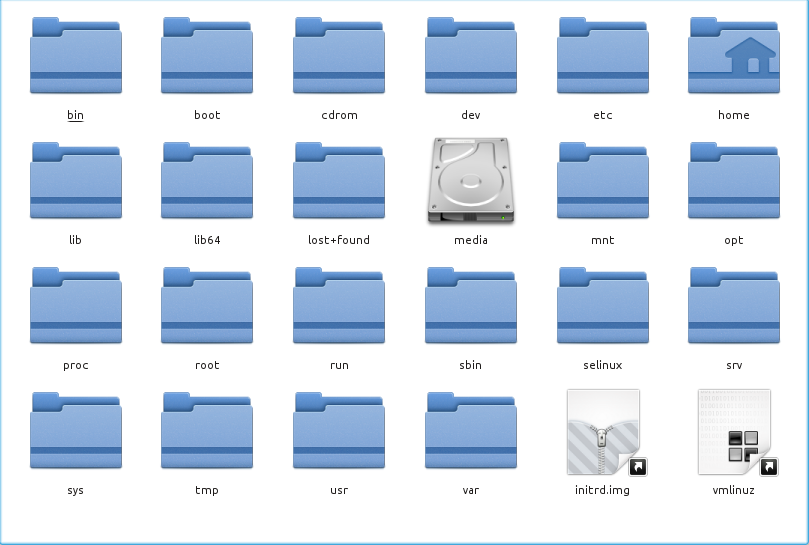
\includegraphics[scale=0.5]{images/Filesystem.png}
		%\caption{}
		%\label{}
	\end{figure}
}

\subsection{Shell}
\frame{\frametitle{Shell}
	\begin{itemize}
		\item Interface between user and kernel
		\item Can be \alert {command line} (eg. Bash, Csh, Zsh, etc.) or can be \alert {graphical} (eg. Gnome, KDE, etc.) 
	\end{itemize}
	\begin{figure}[htp]
		\centering
		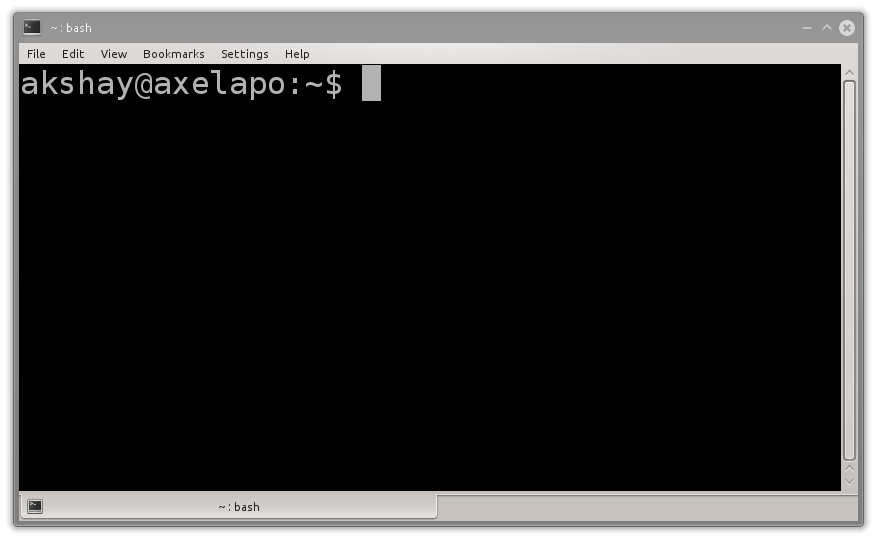
\includegraphics[scale=0.3]{images/bash.png}
		\caption {Bash}
	\end{figure}
}
\begin{comment}
\frame{\frametitle{Bash}
	\begin{itemize}
		\item Bourne Again SHell
		\item Command Line Interface
	\end{itemize}
}
\end{comment}
\subsection{Basic Commands}
\frame{\frametitle{Basic Commands}
	\begin{itemize}
		\item \alert {ls} : List files and directories
		\item \alert {cd} : Change Directory
		\item \alert {pwd} : Print Working Directory
		\item \alert {mkdir} : Make Directory
		\item \alert {cp} : Copy Files
		\item \alert {mv} : Move Files
		\item \alert {rm} : Remove Files
		\item \alert {cat} : Concatenate files and print
		\item \alert {touch} : Change file timestamps
		\item \alert {man} : Read reference manuals
		\item \alert {less} : View files
	\end{itemize}
}
\frame{\frametitle{Special Symbols}
	\begin{itemize}
		\item \alert{*} : All files
		\item \alert{\textbackslash} : Escape Character
		\item \alert{\~{}} : Home
		\item \alert{.} : Current Directory
		\item \alert{.{.}} : Parent Directory
	\end{itemize}
}
\frame{\frametitle{Redirection}
	\begin{itemize}
		\item \alert{\textless} and \alert{\textgreater} : Redirect
		\item \alert{\textless\textless} and \alert{\textgreater\textgreater} : Append
		\item \alert{\textbar} : Pipe
	\end{itemize}
}
\section{Writing Programs}
\subsection{What We Need}
\frame{\frametitle{What We Need}
	\begin{itemize}
		\item \alert {Editor} : gedit, kate, vim, emacs.
		\item \alert {Compiler} : GNU Compiler Collection (gcc)
		\item \alert {Debugger} : GNU Debugger (gdb)
	\end{itemize}
}

\subsection{Write a program}
\frame{\frametitle{Write a program}
	\begin{itemize}
		\item Create directory \alert{/home/student/sum/}
		\item Create a file \alert{sum.c}
		\item Open the File
		\item Write a Program in C to \alert{calculate sum on n numbers}.
	\end{itemize}
}
\frame{\frametitle{Code}
	\lstinputlisting [language=c] {code/sum.c}
}
\subsection{Compile and Run}
\frame{\frametitle{Compile and Run}
	\begin{itemize}
		\item Command to use: gcc
		\item Syntax: gcc [options] input\_file.c
		\item Options
		\begin{itemize}
			\item -o : Output File
			\item -Wall : Show all warnings
			\item -c : Compile Only
		\end{itemize}
		\item Example \\
			\alert {\$ gcc -o sum sum.c}
		\item Run \\
			\alert {\$ ./sum}
	\end{itemize}
}
\section{Debugging Programs}
\subsection{One}
\frame{\frametitle{One}
	abcd
}
% Ending slide is title page again
\section*{}
\frame{\titlepage}
\end{document}
